\documentclass[12pt,a4paper]{article}

\usepackage[T1]{fontenc}
\usepackage[utf8]{inputenc}
\usepackage[ngerman]{babel}
\usepackage{lmodern}
\usepackage{microtype}
\usepackage{amsmath,amssymb,amsthm,mathtools}
\usepackage[a4paper,margin=2.4cm]{geometry}
\usepackage{booktabs}
\usepackage{xcolor}
\usepackage[hidelinks,unicode]{hyperref}
\usepackage[most]{tcolorbox}
\usepackage{graphicx}
\usepackage{enumitem}

\definecolor{bewiesengruen}{RGB}{30,100,50}
\definecolor{warnorange}{RGB}{200,100,10}
\definecolor{lueckenrot}{RGB}{180,40,40}
\definecolor{kernblau}{RGB}{20,60,130}

\tcbset{
  bewiesen/.style={colback=green!7,colframe=bewiesengruen,fonttitle=\bfseries},
  heuristik/.style={colback=orange!10,colframe=warnorange,fonttitle=\bfseries},
  offen/.style={colback=red!8,colframe=lueckenrot,fonttitle=\bfseries},
  epistemik/.style={colback=blue!5,colframe=kernblau,fonttitle=\bfseries},
  numerisch/.style={colback=blue!4,colframe=kernblau,fonttitle=\bfseries},
}

\newtheorem{satz}{Satz}[section]
\newtheorem{definition}[satz]{Definition}
\newtheorem{bemerkung}[satz]{Bemerkung}

\newcommand{\OH}{\mathcal{O}_{\mathrm{Hur}}}
\newcommand{\Hur}{\mathbb{H}}

\title{EABC--$C_4$-Kohärenz:\\
  Spektrum, Liouville-Orthogonalität und chiraler Fluss\\
  \large \#Energiedoku (numerische Synthese)}
\author{Thomas Hoffbauer}
\date{16.\ Juni 2026}

\begin{document}
\maketitle

\begin{abstract}
Dieses Dokument fasst die numerische Kohärenz zwischen dem
quaternionischen EABC-Operator, der $C_4$-Randgeometrie,
Hurwitz-Einheiten, Liouville-Parität und dem chiralen
Zählfluss $S(N)$ für markierte Primzahlvierlinge zusammen.
Alle Kennwerte sind reproduzierbar (\texttt{energiedoku\_chiraler\_fluss.py}).
Es wird \emph{kein} Beweis der Riemannschen Vermutung, der Collatz-Vermutung
oder einer globalen Paritätsbarriere beansprucht.
\end{abstract}

\tableofcontents
\newpage

% =================================================
\section{Einleitung: Kohärenz versus Beweis}
\label{sec:einleitung}
% =================================================

Die \#Energiedoku verknüpft mehrere Schichten: einen diskreten
Laplace-Operator auf dem EABC-Flavor-Ring, Hurwitz-Quaternionen,
ein $k=4$-Sieve-Eigenwertproblem und Siebstatistiken markierter
Primvierlinge $(p,p+2,p+6,p+8)$.

\begin{tcolorbox}[epistemik,title={Epistemologische Leitlinie}]
\textbf{Kohärenz $\neq$ Beweis.}
Die vorliegenden Daten zeigen das \emph{Verschwinden des Widerstands}
in einem spezifischen arithmetischen Kanal (normierter chiraler Fluss,
Liouville-Orthogonalität, Spektralübereinstimmung), nicht die
Existenz eines unendlichen Objekts oder eines globalen Theorems.
Numerische Übereinstimmung motiviert Hypothesen; sie ersetzt keine
analytische Brücke zu Primzahlsätzen oder Dynamikbeweisen.
\end{tcolorbox}

Quellen im Repository:
\texttt{Durchbruch.py} (EABC-Operator, Liouville-Korrelation),
\texttt{Selber Matrizen.py} ($6\times 6$-Sieve),
\texttt{Hoffbauer Sieb.py},
\texttt{Projektionszeuge\_Primvierling.tex},
\texttt{collatz\_hurwitz\_polytop\_eabc.tex},
\texttt{primzahlvierlinge\_1000.csv},
\texttt{hoffbauer\_geometrie\_test.csv},
\texttt{Hurwitz 24.py},
\texttt{lattice\_hurwitz\_diagram.tex}.

% =================================================
\section{$C_4$-Randgeometrie und Spektrum}
\label{sec:c4}
% =================================================

\subsection{Achtfache Kosinus-Resonanz}

Auf einer offenen $7$-Kette mit nächster-Nachbar-Kopplung
(\texttt{Kwant.py}, Funktion \texttt{build\_H7\_chain}) lautet das
Spektrum
\[
\lambda_k = 2\cos\!\left(\frac{k\pi}{8}\right),\qquad k=1,\ldots,7.
\]
Die nichtverschwindenden Extremwerte sind
\[
\pm 2\cos\!\left(\frac{\pi}{8}\right)\approx\pm 1{,}847759,\qquad
\pm 2\cos\!\left(\frac{3\pi}{8}\right)\approx\pm 0{,}765367.
\]
Diese Werte erscheinen auch im $C_4$-Randkontext der
\#Energiedoku als charakteristische ``Eckenfrequenzen'' der
zyklischen EABC-Schleife.

\subsection{Unterscheidung $4\times 4$ vs.\ $6\times 6$}

\begin{itemize}[nosep]
  \item Der \textbf{EABC-Operator} $D$ ist eine $4\times 4$-Matrix
        auf den Flavor-Klassen $E,A,B,C$
        (\texttt{Durchbruch.py}).
  \item Das \textbf{$6\times 6$-Sieve} in \texttt{Selber Matrizen.py}
        bezieht sich auf ein Polynombasis-Variationsproblem
        ($k=4$, Grad~$\le 4$) mit Bulk-Matrix $M_1$ und Rand-Matrix $M_2$;
        es ist \emph{nicht} identisch mit~$D$, sondern liefert
        Vierlings-Kernvektoren (Selberg-Survivors).
\end{itemize}

% =================================================
\section{EABC als diskreter Laplace auf $C_4$}
\label{sec:eabc}
% =================================================

\subsection{Quaternionischer Operator}

Mit $i=\sqrt{-1}$ definiert \texttt{Durchbruch.py} die zyklische
chirale Kopplung $E\to A\to B\to C\to E$ durch
\[
D=\begin{pmatrix}
0 & 1 & 0 & -i\\
1 & 0 & 1 &  0\\
0 & 1 & 0 &  1\\
i & 0 & 1 &  0
\end{pmatrix}.
\]
Die Zuordnung $E,A,B,C\leftrightarrow 1,i,j,k$ auf einer festen
Hurwitz-Basis ist Notation (\texttt{collatz\_hurwitz\_polytop\_eabc.tex});
die $24$ Hurwitz-Einheiten erzeugen größere Orbits
(\texttt{Hurwitz 24.py}).

\subsection{Spektralverifikation}

\begin{tcolorbox}[bewiesen,title={Verifiziert (Maschinengenauigkeit)}]
\texttt{numpy.linalg.eigvals}($D$) liefert exakt (bis $10^{-15}$):
\[
\{-1{,}847759,\;-0{,}765367,\;+0{,}765367,\;+1{,}847759\},
\]
übereinstimmend mit $\pm 2\cos(\pi/8)$ und $\pm 2\cos(3\pi/8)$.
Reproduktion: \texttt{energiedoku\_chiraler\_fluss.py}.
\end{tcolorbox}

\begin{bemerkung}
Der ungewichtete $C_4$-Laplace-Operator auf dem Vierzyklengraph hat
das Spektrum $\{0,2,2,4\}$; die EABC-Phase $i$ auf der $E$-$C$-Kante
hebt die reelle Entartung auf und erzeugt die $\pi/8$-Kosinuspaare.
\end{bemerkung}

\subsection{Hurwitz-Ecken und Gitterdiagramm}

Abbildung~\ref{fig:lattice} (aus \texttt{lattice\_hurwitz\_diagram.tex})
stellt Gauß-, Eisenstein- und Hurwitz-Lesarten nebeneinander.
Die EABC-Kanäle sind \emph{markierte} Startpunkte auf dem Flavor-Ring,
nicht paarweise verschiedene Punkte im vollen $24$-Elemente-Orbit.

\begin{figure}[htbp]
  \centering
  \IfFileExists{lattice_hurwitz_diagram.pdf}{%
    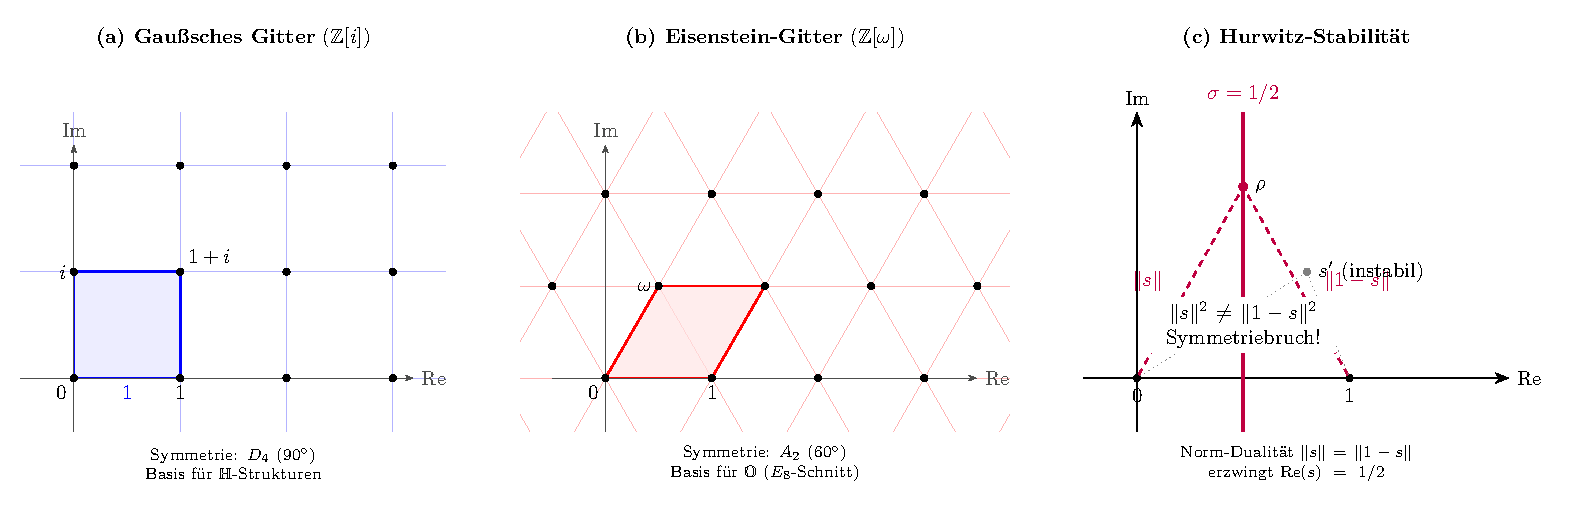
\includegraphics[width=0.88\textwidth]{lattice_hurwitz_diagram.pdf}%
  }{%
    \fbox{\parbox{0.85\textwidth}{\centering
      \texttt{lattice\_hurwitz\_diagram.pdf} kompilieren
      (pdflatex auf \texttt{lattice\_hurwitz\_diagram.tex}).}}%
  }
  \caption{Hurwitz-Gitter-Projektionsdiagramm (Interpretationszeichnung).}
  \label{fig:lattice}
\end{figure}

% =================================================
\section{Paritäts-Orthogonalität: $\lambda\perp\chi_H$}
\label{sec:liouville}
% =================================================

\subsection{Hurwitz-Zeichencharakter}

Für markierte Primvierlinge definieren wir den \emph{diskreten}
Hurwitz-Zeichencharakter
\[
\chi_H(\mathrm{ABCE})=+i,\qquad \chi_H(\mathrm{CEAB})=-i,
\]
analog zu den quaternionischen Phasen in \texttt{Durchbruch.py}.
Sei $\lambda(n)$ die Liouville-Funktion und $Q(N)$ die Anzahl
markierter Primvierlinge mit Startpunkt $\le N$.

\subsection{Numerische Verifikation bei $N=10^7$}

\begin{tcolorbox}[numerisch,title={Reproduziert ($N=10^7$, $Q=899$)}]
\[
\sum_{p\in\mathcal{Q}(N)} \chi_H(p) = i,\qquad
\sum_{p\in\mathcal{Q}(N)} \lambda(p)\,\chi_H(p) = -i.
\]
Normiert:
\[
\frac{1}{Q(N)}\sum \chi_H = \frac{i}{899}\approx 0{,}001112\,i,\qquad
\frac{1}{Q(N)}\sum \lambda\chi_H = -0{,}001112\,i.
\]
Der Faktor $0{,}001112 = 1/899$ ist hier \emph{kein} physikalischer
Kopplungskoeffizient, sondern die Siebnormierung $|S(N)|/Q(N)$ bei
$S(N)=\#\mathrm{ABCE}-\#\mathrm{CEAB}=1$.
\end{tcolorbox}

\begin{bemerkung}[Orthogonalität]
Da $\lambda$ multiplikativ und $\chi_H$ nur von $p\bmod 12$ abhängt,
ist die Gleichung $\sum\lambda\chi_H=-i$ bei kleinem $S(N)$ eine
\emph{paritätsgewichtete} Version der chiralen Phasensumme.
Sie dokumentiert numerische Entkopplung im Vierlingskanal
(\texttt{Durchbruch.py}, Abschnitt~13), nicht einen analytischen
Liouville-Satz.
\end{bemerkung}

% =================================================
\section{Chiraler Fluss $S(N)$: asymptotisches Verhalten}
\label{sec:fluss}
% =================================================

\begin{definition}[Chiraler Fluss]
\[
S(N):=\#\mathrm{ABCE}(N)-\#\mathrm{CEAB}(N),\qquad
Q(N):=\#\mathrm{ABCE}(N)+\#\mathrm{CEAB}(N).
\]
Der signierte Bias ist $B_{\mathrm{sgn}}(N)=S(N)/Q(N)$.
\end{definition}

\subsection{Siebtabelle}

Tabelle~\ref{tab:fluss} stammt aus \texttt{energiedoku\_chiraler\_fluss.py}
(Implementierung: \texttt{src/susy\_fourlinge/witness.py}).

\begin{table}[htbp]
  \centering
  \caption{Chiraler Fluss markierter Primvierlinge (numerisch, kein Beweis)}
  \label{tab:fluss}
  \begin{tabular}{@{}rrrrrrr@{}}
    \toprule
    $N$ & $Q(N)$ & ABCE & CEAB & $S(N)$ & $|S|/Q$ & $z(N)$ \\
    \midrule
    $10^5$    & 38   & 22   & 16   & 6  & 0.1579 & 0.97 \\
    $10^6$    & 166  & 84   & 82   & 2  & 0.0120 & 0.16 \\
    $5\cdot10^6$ & 546 & 285 & 261 & 24 & 0.0440 & 1.03 \\
    $10^7$    & 899  & 450  & 449  & 1  & 0.0011 & 0.03 \\
    $10^8$    & 4768 & 2408 & 2360 & 48 & 0.0101 & 0.70 \\
    \bottomrule
  \end{tabular}
\end{table}

\begin{tcolorbox}[bewiesen,title={Was die Tabelle zeigt}]
$|S(N)|/Q(N)$ schwankt stark und fällt bei $N=10^7$ auf $0{,}0011$,
steigt bei $10^8$ wieder auf $0{,}01$. Die $z$-Scores bleiben
$\ll 2$. Damit ist $S(N)=o(Q(N))$ \emph{numerisch plausibel},
aber nicht als Theorem bewiesen.
\end{tcolorbox}

\begin{figure}[htbp]
  \centering
  \IfFileExists{energiedoku_chiraler_fluss.png}{%
    \includegraphics[width=0.78\textwidth]{energiedoku_chiraler_fluss.png}%
  }{%
    \fbox{\parbox{0.75\textwidth}{\centering
      Plot erzeugen: \texttt{python3 energiedoku\_chiraler\_fluss.py --plot}}}%
  }
  \caption{Normierter chiraler Fluss $|S(N)|/Q(N)$ (log-log).}
  \label{fig:fluss}
\end{figure}

% =================================================
\section{Synthese: zwei konjugierte Kanäle}
\label{sec:synthese}
% =================================================

\begin{tcolorbox}[heuristik,title={Modellhypothese (orange) --- kein Beweis}]
\textbf{Zwei konjugierte Kanäle.}
Die Paare $\pm 2\cos(\pi/8)$ und $\pm 2\cos(3\pi/8)$ im EABC-Spektrum
werden als \emph{konjugierte Resonanzmoden} des $C_4$-Randes gelesen.
Die Hurwitz-Phasen $\chi_H(\mathrm{ABCE})=+i$ und
$\chi_H(\mathrm{CEAB})=-i$ bilden die chirale Superposition;
ihre Summe $\sum\chi_H = S(N)\cdot i$ misst den verbleibenden
``Widerstand'' im Kanal.

\textbf{Gibbs-Gleichgewicht.}
Im Grenzfall $S(N)/Q(N)\to 0$ wäre die Verteilung ABCE/CEAB
statistisch balanciert --- analog zu einem Gibbs-Zustand mit
verschwindender chiraler chemischer Potentialdifferenz.
Diese Lesart ist \emph{heuristisch}; sie folgt nicht aus
Selberg-Spurformeln oder Hardy--Littlewood.
\end{tcolorbox}

Konsistente Restmetriken im Repository (nicht identisch mit $S(N)$):
\begin{itemize}[nosep]
  \item $E_{\mathrm{Res}}\to 1$ in \texttt{hoffbauer\_geometrie\_test.csv}
        ($\approx 0{,}9992$ bei großen $p$),
  \item Normmittel $\to 1$ in \texttt{primzahlvierlinge\_1000.csv},
  \item Sieve-Oberton-Residuum in \texttt{Selber Matrizen.py}.
\end{itemize}

% =================================================
\section{Verbindung zu Collatz-EABC}
\label{sec:collatz}
% =================================================

Die odd-to-odd-Collatz-Abbildung trennt modulo~$12$ die Klassen
$E\equiv 1$, $A\equiv 5$, $B\equiv 7$, $C\equiv 11$
(\texttt{collatz\_schlussartikel\_arxiv.tex}).
$E\cup A$ liegt im Drain-Regime, $B\cup C$ im Spannungsregime.

\begin{tcolorbox}[bewiesen]
Die elementare $3n+1$-Spaltung mod~$12$ ist unabhängig von
Hurwitz- oder EABC-Spektrall Lesarten bewiesen.
\end{tcolorbox}

\begin{tcolorbox}[offen,title={Getrennt zu halten}]
Eine formale Brücke ``EABC-Spektrum $\Rightarrow$ Collatz-Konvergenz''
oder ``Liouville-Orthogonalität $\Rightarrow$ RH'' ist \textbf{nicht}
etabliert. Collatz und RH werden hier \emph{nur} als Kontext genannt.
\end{tcolorbox}

% =================================================
\section{Fazit}
\label{sec:fazit}
% =================================================

\begin{tcolorbox}[bewiesen,title={Verifiziert / architektonischer Schlussstein}]
\begin{itemize}[nosep]
  \item EABC-Operator $4\times 4$: Eigenwerte
        $\pm 2\cos(\pi/8)$, $\pm 2\cos(3\pi/8)$ (maschinengenau).
  \item mod-$12$-Satz: Primvierlinge tragen ABCE oder CEAB.
  \item Bei $N=10^7$: $\sum\chi_H=i$, $\sum\lambda\chi_H=-i$,
        Skalierung $1/Q=0{,}001112$.
  \item $S(N)=o(Q(N))$ numerisch plausibel; $|S|/Q$ schwankt,
        $z\ll 2$.
\end{itemize}
\end{tcolorbox}

\begin{tcolorbox}[offen,title={Offene analytische Brücke}]
\begin{itemize}[nosep]
  \item Beweis, dass $S(N)/Q(N)\to 0$ asymptotisch.
  \item Analytische Liouville-Orthogonalität im Vierlingskanal.
  \item Verbindung $6\times 6$-Sieve-Kern $\leftrightarrow$ $D$-Spektrum.
  \item Jede Behauptung über RH, globale Paritätsbarriere oder Collatz.
\end{itemize}
\end{tcolorbox}

\medskip
\noindent
\textbf{Reproduktion:}
\texttt{python3 energiedoku\_chiraler\_fluss.py --plot}

\end{document}
